\section{Results}
\label{sec:results}
Unless stated otherwise, results are for the public V-JEPA ViT-L checkpoint (M1) on the 180 IntPhys dev pairs. Percentages use the tie-half convention (Section~\ref{sec:method}); strict-convention values are given where they differ. Confidence intervals are 95\% scene-cluster bootstrap intervals. Under the pre-registered rules, H1 (invariance) is descriptive for M1, H2 (specificity) is detection-limited, and gate G2 was not met; read every statement below with that in mind.

\subsection{Clean accuracy and baselines}
\label{sec:res-clean}
Clean pairwise accuracy of M1 is 81.7\% in fp32 (80.6\% strict) and 80.8\% in fp16 (81.1\% strict); the fp16 run is the reference for all contrasts. The published 98\% (ViT-H) is not reproduced (Section~\ref{sec:deviations}). The public ViT-H checkpoint, the like-for-like comparison, reaches 88.3\% (87.8\% strict). The copy-last-frame baseline B2 reaches 76.1\%, and the windowed frame-difference baseline B1 reaches 58.1\% (57.2\% strict). The paired difference between M1 (fp16) and B2 is +4.7 pp with a confidence interval of $-$1.1 to 10.6 pp, which includes zero; against the fp32 run it is +5.6 pp (0.0 to 11.1), with the lower bound at zero. Clean accuracy does not separate M1 from a copy-last-frame pixel baseline. V-JEPA~2 (M2) reaches 60.8\% after the mask-token correction (60.6\% strict; 46.9\% before it) and is not H1-eligible. VideoMAE~V2 (M3) was not run. Table~\ref{tab:t1} lists all rows.

\IfFileExists{tables/t1_reproduction.tex}{\begin{table}[t]
\caption{Reproduction on IntPhys dev (180 pairs, 3 blocks): pairwise accuracy in \% of the impossible video having the higher surprise (mean aggregation; tie-half = primary, strict = ties counted wrong). Published: Garrido et al.\ headline $\approx$98\%, obtained with checkpoints that are not released; the gap to our public checkpoints is unexplained and we make no reproduction claim. M1 minus B2 (paired): +4.7 pp [$-$1.1, 10.6].}
\label{tab:t1}
\centering\scriptsize
\setlength{\tabcolsep}{2.5pt}
\begin{tabular}{@{}lrrr@{}}
\toprule
Model & Tie-half & Strict & Published \\
\midrule
M1 V-JEPA ViT-L, fp32 & 81.7 & 80.6 & $\approx$98$^{\rm a}$ \\
M1 V-JEPA ViT-L, fp16 & 80.8 & 81.1 & -- \\
M1H V-JEPA ViT-H (diagn.)$^{\rm b}$ & 88.3 & 87.8 & -- \\
M2 V-JEPA 2 ViT-L & 60.8 & 60.6 & -- \\
M3 VideoMAE V2 & \multicolumn{2}{c}{\textit{not run}} & -- \\
M0r random init (3) & 50.0 & 50.2 & expected $\approx$50 \\
B1 frame difference & 58.1 & 57.2 & expected $\approx$50 \\
B2 copy-last-frame & 76.1 & 76.1 & -- \\
\midrule
\multicolumn{4}{@{}l}{\textit{Superseded, disclosure only (not the M2 number)}} \\
M2 old run (mask idx 1)$^{\rm c}$ & 46.9 & 46.7 & -- \\
\bottomrule
\end{tabular}
\vspace{2pt}

\raggedright\scriptsize $^{\rm a}$Literature value, not our run. $^{\rm b}$Prereg-tau tie-half 88.3; the 88.1 in the pre-registration text is the superseded fixed-$\tau$ figure (strict 87.8). $^{\rm c}$Wrapper deviation (query mask index 1), excluded from every M2 contrast.
\end{table}
}{\par\noindent\textbf{[TODO table T1: tables/t1\_reproduction.tex missing]}\par}

\subsection{Invariance (H1): descriptive}
\label{sec:res-h1}
The verdict flip rate under an imperceptible $\pm1$ grey-level dither is 21.5\% (15.6\% strict), above the 10\% limit, so invariance for M1 is descriptive and we report accuracy changes and flip rates relative to this floor (Table~\ref{tab:t2}; Fig.~S1 in the supplement). We do not assign the driver's verdict labels. At high strength, additive noise lowers accuracy by $-$20.6 pp ($-$25.7 to $-$15.3) with a flip rate of 37.8\%, +16.3 pp above the floor (10.6 to 22.4). Blur lowers accuracy by $-$14.4 pp ($-$19.4 to $-$9.4; flip 31.1\%, +9.6 pp above the floor), and JPEG by $-$10.8 pp ($-$16.4 to $-$5.3; flip 28.3\%, +6.9 pp above the floor). For JPEG the Holm-adjusted accuracy test depends on the convention: under tie-half the cluster and sign tests give $p$ $<$0.0001 and 0.018, under the strict convention 0.0088 and 0.1151. Brightness changes accuracy by $-$2.4 pp ($-$5.1 to 0.3; flip 12.4\%), horizontal flip by +2.2 pp ($-$2.2 to 6.7; flip 15.0\%) and centre crop by $-$0.5 pp ($-$5.7 to 4.9; flip 14.3\%, on 112 of 180 pairs after the retention exclusion). For these three, the flip rate is at or below the dither floor, so the edit adds no flips beyond the floor. The frame-rate edit is bit-identical to its reference by a design error and tests nothing; it is excluded here.

\emph{Dose-response (A3, descriptive).} Accuracy loss grows with strength for blur ($-$4.7, $-$11.9, $-$14.4 pp at low, mid, high); for JPEG the change is +5.8, +0.8 and $-$10.8 pp, so a loss appears only at the highest setting. Noise is already at $-$17.7 pp at the lowest strength (flip 33.2\%), and brightness stays within a few points of zero at all strengths, with low- and mid-strength flip rates (7.0\% and 9.6\%) below the floor. The family is Holm over 30 tests (Section~\ref{sec:deviations}; Table~S4 and Fig.~S2 in the supplement).

\IfFileExists{tables/t2_invariance.tex}{\begin{table*}[t]
\caption{Invariance (H1), high strength. $\Delta$Acc = accuracy under the same edit applied to both videos of a pair minus clean accuracy, in percentage points (scene-cluster 95\% CI); flip = share of pairs whose verdict changes; flip$-f_0$ = flip rate minus the dither floor $f_0$ (a perturbation that should not matter at all): M1 $f_0$ = 21.5\% (strict 15.6\%), M2 $f_0$ = 24.6\%. A flip rate near $f_0$ is what an invisible perturbation produces. Holm-14 adjusted $p$ for $\Delta$Acc / flip. M1 is the confirmatory row; M2 is \textbf{descriptive only} (clean accuracy below the 80\% eligibility rule).}
\label{tab:t2}
\centering\scriptsize
\setlength{\tabcolsep}{1.9pt}
\begin{tabular}{@{}lrrrrrrrr@{}}
\toprule
 & \multicolumn{4}{c}{M1 V-JEPA ViT-L} & \multicolumn{4}{c}{M2 V-JEPA 2 (descriptive)} \\
\cmidrule(lr){2-5}\cmidrule(lr){6-9}
Edit ($n$ pairs) & $\Delta$Acc [CI] & Flip & Flip$-f_0$ [CI] & $p$ ($\Delta$/flip) & $\Delta$Acc [CI] & Flip & Flip$-f_0$ [CI] & $p$ ($\Delta$/flip) \\
\midrule
Brightness (180) & $-$2.4 [$-$5.1, 0.3] & 12.4 & $-$9.1 [$-$14.1, $-$4.4] & 0.63 / 1.00 & $-$0.4 [$-$3.1, 2.5] & 15.4 & $-$9.3 [$-$14.3, $-$4.6] & 1.00 / 1.00 \\
Noise (180) & $-$20.6 [$-$25.7, $-$15.3] & 37.8 & +16.3 [10.6, 22.4] & $<$0.001 / $<$0.001 & $-$6.4 [$-$11.5, $-$1.3] & 28.3 & +3.7 [$-$0.2, 8.0] & 0.13 / 0.30 \\
Blur (180) & $-$14.4 [$-$19.4, $-$9.4] & 31.1 & +9.6 [4.3, 15.4] & $<$0.001 / 0.001 & +12.8 [6.4, 19.2] & 42.2 & +17.6 [10.4, 24.8] & $<$0.001 / $<$0.001 \\
JPEG (180) & $-$10.8 [$-$16.4, $-$5.3] & 28.3 & +6.9 [0.6, 13.7] & $<$0.001 / 0.15 & $-$1.7 [$-$7.8, 4.4] & 40.6 & +15.9 [8.9, 23.3] & 1.00 / $<$0.001 \\
Zoom (crop)$^{\rm a}$ (112) & $-$0.5 [$-$5.7, 4.9] & 14.3 & $-$8.9 [$-$16.4, $-$1.6] & 1.00 / 1.00 & +7.1 [1.7, 12.8] & 25.0 & $-$5.7 [$-$13.9, 3.1] & 0.13 / 1.00 \\
Horiz.\ flip (180) & +2.2 [$-$2.2, 6.7] & 15.0 & $-$6.5 [$-$12.8, $-$0.2] & 1.00 / 1.00 & +3.3 [$-$0.3, 6.9] & 15.6 & $-$9.1 [$-$14.1, $-$4.1] & 0.58 / 1.00 \\
\bottomrule
\end{tabular}

\vspace{2pt}
\raggedright\scriptsize Flip and flip$-f_0$ in \%, $\Delta$Acc in pp. $^{\rm a}$Pairs where the crop keeps the scene support (112 of 180); the other 68 are excluded for both models. Frame-rate halving is not tabulated: its edited input is bit-identical to the skip-4 clean reference, so the edit is degenerate by design (a design error in the edit list, reported here for completeness).
\end{table*}
}{\par\noindent\textbf{[TODO table T2: tables/t2\_invariance.tex missing]}\par}

\subsection{Positive controls (H3, gate G2): not met}
\label{sec:res-h3}
Vertical flip raises M1's surprise in 21.1\% of possible videos (14.7 to 28.1), far below the 80\% gate; against the horizontal-flip reference the rate is 25.8\% (18.6 to 33.3). Horizontal flip itself gives 38.6\%. Time reversal, reported but not gating, gives 60.8\% (51.7 to 69.4). Pairwise accuracy on vertically flipped pairs is 83.9\%, not lower than the clean 80.8\%. The random-weight network M0r raises its surprise under vertical flip in 87.8\% of videos (82.2 to 93.1), where the pre-registration expected about 50\%; the M1 minus M0r difference in detection is $-$66.7 pp ($-$76.1 to $-$56.7), and we do not interpret it as a measure of learned sensitivity. G2 was not met. We cannot show that the pipeline responds to physical violations other than the dataset's own frame splices (Table~S2 in the supplement).

\subsection{Specificity (H2): detection-limited}
\label{sec:res-h2}
The test uses the 180 possible videos. The event rule fell back to a random onset in 178 of 180 pairs, and the median matched magnitude is 0.33 grey levels of 255, so the edits are near-threshold. For global lighting, 84 of 180 entries are no-ops after rounding. The specificity AUROC of M1 is $A=$0.546 (0.501 to 0.591), and 0.520 (0.475 to 0.565) without global lighting. Per type it is 0.622 (global lighting), 0.480 (local lighting), 0.553 (camera jolt) and 0.528 (zoom); the global-lighting value largely measures clean detection and is not evidence of partial specificity. The detection precondition is not met: clean accuracy under the same aggregation is $A_0=$0.722 (0.664 to 0.781) against the required 0.85. By the pre-registered rule the outcome is \emph{detection-limited}: specificity cannot be assessed here and we make no claim in either direction. The outcome is the same under the strict and exact-tie conventions and with global lighting excluded. Ablations over aggregation and fixed context length are in Supplement Table~S5, and results per block in Table~S6.

Both pixel baselines fall below chance, with $A_{B1}=$0.335 and $A_{B2}=$0.379. The contrasts $D_1=$+0.211 (0.159 to 0.263) and $D_2=$+0.166 (0.116 to 0.219) are Holm-significant ($p=$0.0002, the bootstrap floor), but this reflects the baselines' distance below 0.5 under this matching, not evidence about M1; we do not read them as M1 outperforming a baseline. As a function of edit strength, $A$ is 0.594 (0.546 to 0.642) at half the matched magnitude, 0.546 at the matched magnitude and 0.501 (0.458 to 0.543) at twice, and it falls with strength in all four types (descriptive; Holm over 24 tests, all at the bootstrap floor). Figure~\ref{fig:f2} shows the distributions, and Table~S3 in the supplement lists the per-type values, the M2 rows and the analysis without global lighting.

\IfFileExists{figures/f2_specificity.pdf}{\begin{figure*}[t]\centering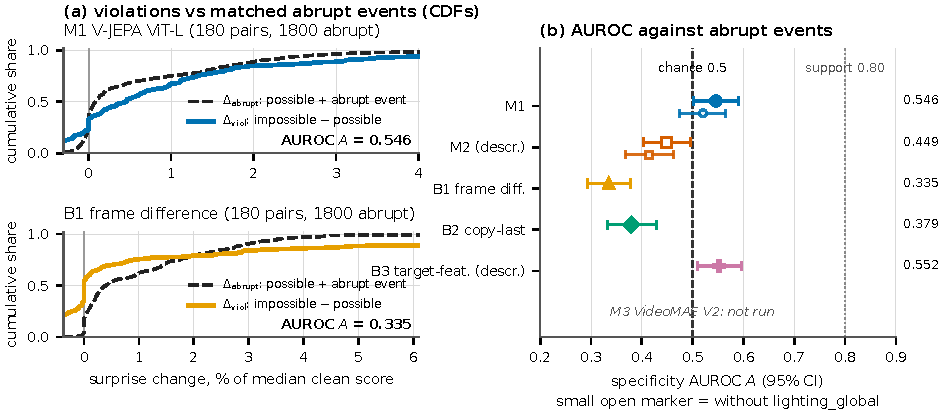
\includegraphics[width=\textwidth]{figures/f2_specificity.pdf}\caption{Specificity (H2) for M1 and the pixel baselines: distributions of $\Delta_{\mathrm{viol}}$ and $\Delta_{\mathrm{abrupt}}$, and AUROC with 95\% intervals. Baselines below 0.5 reflect the matching, not model skill.}\label{fig:f2}\end{figure*}}{\par\noindent\textbf{[TODO figure F2: figures/f2\_specificity.pdf missing]}\par}

\subsection{V-JEPA~2 (M2): descriptive}
\label{sec:res-m2}
M2 is H1-ineligible (clean 60.8\%), so all M2 results are descriptive. Its dither floor is 24.6\%. Its specificity AUROC is 0.449 (0.403 to 0.496), 0.415 without global lighting, with $A_0=$0.600 (0.542 to 0.658); the rule again gives the detection-limited outcome, and the upper interval bound lies below 0.5. Both pixel baselines are again below 0.5 (0.324 and 0.376).

\emph{M2 positive controls.} Vertical flip raises M2's surprise in 71.9\% of videos (64.4 to 78.9), reversal in 46.4\% (38.6 to 54.2); G2 is not met for M2 either, and M2 minus M0r is $-$15.8 pp ($-$25.0 to $-$6.7). Pairwise accuracy on its vertically flipped pairs is 64.4\%. The M2 dose-response (seed 1 only, descriptive) is in Supplement Section~S-II. Because M2 is ineligible and does not meet G2, no statement here extends to latent world models in general.

\subsection{IntPhys 2 Main: descriptive}
\label{sec:res-ip2}
On the 506 IntPhys~2 Main pairs, M1's clean accuracy is 47.6\% (43.7 to 51.7; 47.8\% strict), at chance. The pixel baselines are also at chance (B1 51.2\%, B2 51.9\%, B3 46.6\%). By category M1 scores 46.7\% (continuity), 42.1\% (immutability), 49.6\% (permanence) and 51.4\% (solidity). Removing the four pairs whose names overlap the Debug split changes nothing material (47.6\%). The verdict is at chance here, which limits what the signal can show; we draw no further conclusion from it. We did not run the specificity test on this split (no event-time annotation).

\subsection{Exploratory analyses}
\label{sec:res-expl}
These were run after the confirmatory results were seen and are exploratory (details and Table~S1 in Supplement Section~S-II). An onset-aligned specificity variant, using the splice time derived from prefix-sharing frames of the dev pixels, gives an AUROC for M1 of 0.392 (0.354 to 0.428), lower than with random windows (0.546), with the detection precondition unchanged ($A_0=$0.722), so the rule's outcome does not change; both baselines stay below 0.5. An AUROC below 0.5 means that the matched possible edits raise surprise more than the violations do. M2's AUROC (0.449, upper bound 0.496) is also below 0.5. Under the frozen table this pattern carries the sub-label ``Reversed''; because the detection precondition is unmet, the confirmatory M1 outcome stays detection-limited and we draw no conclusion from it. A hold-based frame-rate edit that differs from the skip-4 reference changes accuracy by +1.9 pp ($-$3.3 to 7.5) with a flip rate of 20.0\%, within the 21.5\% floor. The fp32 flip rate was not measured. A paired check on the stored arrays shows that M0r's surprise shifts systematically in one direction under vertical flip, opposite to M1's shift, and not through ties or noise; the cause is not established.
